% !TeX root = orbits.tex

\section{Lagrange points}\label{s.lagrange}

Consider a spacecraft orbiting the Sun and subject to the gravitational force of both the Earth and the Sun. Joseph-Louis Lagrange and Leonhard Euler discovered that there are five points where the spacecraft rotates with the same orbital period as the Earth and thus appears to maintain a fixed position as viewed from the Earth. These points are called the \emph{Lagrange points} $L1, L2, L3, L4, L5$ and their positions are shown in Figure~\ref{f.lagrangepoints}.\footnote{The orbits are clearly shown in the gif in the Wikipedia entry \emph{Lagrange point}.}

In this section we present an approximate derivation of the locations of $L1, L2, L3$. The most significant approximation is that we assume that the spacecraft orbits around the center of the Sun, whereas it actually orbits around the barycenter of the Sun and the Earth. The derivation of the locations of $L4, L5$ is beyond the scope of this document. The final subsection describes the objects that exist at the Lagrange points.

\begin{figure}[b]
\begin{center}
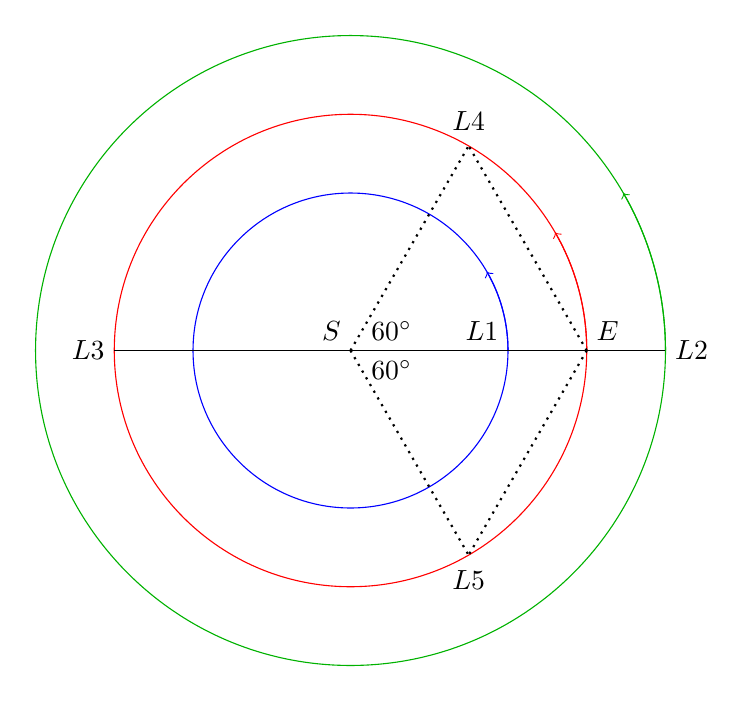
\begin{tikzpicture}
\clip (-4.1,-4.3) rectangle +(8.7,8.4);
\def\re{3}
\def\rone{2}
\def\rtwo{4}
\coordinate (S) at (0,0);
\node[above left] at (S) {$S$};
\vertexsm{S};
\draw[red] (S) circle[radius=\re];
\draw[->,red] ({\re},0) arc[start angle=0, end angle=30, radius=\re];
\draw[blue] (S) circle[radius=\rone];
\draw[->,blue] ({\rone},0) arc[start angle=0, end angle=30, radius=\rone];
\draw[green!70!black] (S) circle[radius=\rtwo];
\draw[->,green!70!black] ({\rtwo},0) 
  arc[start angle=0, end angle=30, radius=\rtwo];
\coordinate (E) at ({\re},0);
\node[above right] at (E) {$E$};
\vertexsm{E};
\coordinate (L1) at ({\rone},0);
\node[above left] at (L1) {$L1$};
\vertexsm{L1};
\coordinate (L2) at ({\rtwo},0);
\node[right] at (L2) {$L2$};
\vertexsm{L2};
\coordinate (L3) at ({-\re},0);
\node[left] at (L3) {$L3$};
\vertexsm{L3};
\draw[dotted,thick] (S) -- +(60:{\re}) coordinate (L4);
\draw[dotted,thick] (E) -- (L4);
\node[above,yshift=2pt] at (L4) {$L4$};
\vertexsm{L4};
\draw[dotted,thick] (S) -- +(-60:{\re}) coordinate (L5);
\draw[dotted,thick] (E) -- (L5);
\node[below,yshift=-2pt] at (L5) {$L5$};
\vertexsm{L5};
\draw (L3) -- (L2);
\node[above right,xshift=4pt] at (S) {$60^\circ$};
\node[below right,xshift=4pt] at (S) {$60^\circ$};
\end{tikzpicture}
\end{center}
\caption{The five Lagrange points}\label{f.lagrangepoints}
\end{figure}

\subsection{Lagrange point $L1$}

We assume that the Earth is in a circular orbit of radius $r_E$ around the Sun and that the masses of the two satisfy $m_S \gg m_E$. Let us suppose that we wish to place a space telescope $T$ of mass $m_T \ll m_E$ in a circular orbit at distance $r_1\ll r_E$ from the Earth (Figure~\ref{f.lagrange1}). Furthermore, let us suppose that we want $T$ to have the same orbital period as the Earth (one year) so that it will be possible to easily receive data at ground stations. Is this possible?

\begin{figure}
\begin{center}
\begin{tikzpicture}
\clip (-.5,-1) rectangle +(7,2);
\def\re{6}
\def\rone{4}
\coordinate (S) at (0,0);
\node[above left] at (S) {$S$};
\vertexsm{S};
\draw[red] (S) circle[radius=\re];
\draw[blue] (S) circle[radius=\rone];
\coordinate (E) at ({\re},0);
\node[above right] at (E) {$E$};
\vertexsm{E};
\coordinate (L1) at ({\rone},0);
\node[above left] at (L1) {$L1$};
\vertexsm{L1};
\draw (S) -- node[fill=white] {$r'=r_E-r_1$} (L1) --
  node[fill=white] {$r_1$} (E);
\draw[<->] ($(S)+(0,-16pt)$) --
  node[fill=white] {$r_E$} ($(E)+(0,-16pt)$);
\end{tikzpicture}
\end{center}
\caption{Lagrange point $L1$}\label{f.lagrange1}
\end{figure}
If we ignore the gravitational force exerted by $E$ on $T$ at $L1$, obviously not, because by Kepler's third law
\[
\frac{A_E^3}{T_E^2} = \frac{A_1^3}{T_1^2}=\frac{A_1^3}{T_E^2}\,,
\]
so $A_1=A_E$ and $T$ must be located at the center of the Earth. Is is possible that the gravitational force exerted by $E$ on $T$ can cause $T_1=T_E$ while $r_1$ is greater than the radius of the Earth?

You might think that $T$ should be placed so that the gravitational force exerted by the Sun is exactly balanced by the gravitational force exerted by the Earth, but, of course, if there is no net force on $T$, by Newton's first law $T$ would simply move in a straight line of into space. Instead, we want the net centripetal force on $T$ to be
\begin{equation}
F = \frac{Gm_Sm_T}{r'^2}-\frac{Gm_Em_T}{r_1^2}\,,\label{eqn.force-diff}
\end{equation}
so that it moves in an orbit with period $T_E$. To simplify notation we let $r'=r_E-r_1$.

Since the length of the orbit of $T$ at $L1$ is $2\pi r'$, $T$'s velocity is
\begin{equation}
v_1 = \frac{2\pi r'}{T_1}\,.\label{eqn.velocity}
\end{equation}
As Newton did in his investigation of elliptical orbits, in Figure~\ref{f.grav-lagrange} the motion from $A$ to $D$ is separated into the tangential motion $AC$ where there is no force on $T$, followed by motion towards the center with a centripetal force from $C$ to $S$. The distances indicated are those of the non-accelerated $v_t\Delta t$ and the accelerated motion $\frac{1}{2} a (\Delta t)^2$ during a very small time period $\Delta t$. We need to find the acceleration $a$ that will cause $T$ to reach $D$.
\begin{figure}[t]
\begin{center}
\begin{tikzpicture}
\clip (-5.5,-.5) rectangle +(6,5);

\def\r{4}
\coordinate (S) at (0,0);
\node[below] at (S) {$S$};
\coordinate (A) at (0,{\r});
\node[above] at (A) {$A$};
\draw (0,{\r}) arc(90:180:{\r});
\draw (S) -- node[right] {$r'$} (A);
\coordinate (D) at (140:{\r});
\node[below,yshift=-4pt] at (D) {$D$};
\path[name path=radius] (S) -- (140:{2*\r});
\path[name path=ac] (A) -- +({-1.5*\r},0);
\path [name intersections = {of = radius and ac, by = {C} }];
\node[above] at (C) {$C$};
\draw[->] (A) -- node[above] {$v_1\Delta t$} (C);
\draw[->] (C) -- node[right,xshift=2pt] {$x$} 
  node[left,xshift=-4pt,yshift=-2pt] {$\frac{1}{2} a (\Delta t)^2$} (D);
\draw (S) -- node[left,xshift=-4pt] {$r'$} (D);
\draw[->] (A) arc (90:120:{\r});
\end{tikzpicture}
\caption{Non-accelerated and accelerated motion}\label{f.grav-lagrange}
\end{center}
\end{figure}
Applying Pythagoras's theorem we get
\begin{eqn}
r'^2 + (v_1\Delta t)^2 &=& (r'+x)^2 =r'^2 + 2r'x + x^2\\
(v_1\Delta t)^2 &=& x(2r'+x)\,.
\end{eqn}%
Since $\Delta t$ is assumed to be a very small time interval and since $r_T$ is close to $r_E$, $2r'+x \approx 2r'$ so using the definition of $x$, from Newton's second law we have
\begin{eqn}
\frac{1}{2} a (\Delta t)^2 &=& \frac{1}{2}\frac{v_1^2}{r'}(\Delta t)^2\\
F &=& m_T a = \frac{m_Tv_1^2}{r'}\,.
\end{eqn}%
By Equation~\ref{eqn.force-diff} the force needed to keep $T$ in the desired orbit is
\[
F=\frac{m_Tv_T^2}{r'} = \frac{Gm_Sm_T}{r'^2}-\frac{Gm_Em_T}{r_1^2}\,,
\]
so the velocity of $T$ at $L1$ must satisfy
\[
v_1^2= \frac{Gm_S}{r'}-\frac{Gm_Er'}{r_1^2}\,.
\]
The period of the desired orbit is $T_1=T_E$ so using Equation~\ref{eqn.velocity}, we get
\begin{eqn}
\frac{4\pi^2 r'^2}{T_E^2}&=&\frac{Gm_S}{r'}-\frac{Gm_Er'}{r_t^2}\\
\frac{4\pi^2}{T_E^2}&=&\frac{Gm_S}{r'^3}-\frac{Gm_E}{r'r_t^2}\,.
\end{eqn}%
But by Kepler's third law (Equation~\ref{eqn.third-law}), where the elliptical semi-major axis $a_i$ is the circular radius $r_E$,
\begin{eqnlabels}
\frac{4\pi^2 r_E^3 m}{T_E^2}\frac{1}{r_E^2}&=&\frac{GmM}{r_E^2}\nonumber\\
\frac{Gm_S}{r_E^3}&=&\frac{Gm_S}{r'^3}-\frac{Gm_E}{r'r_1^2}\nonumber\\
\frac{1}{r_E^3}&=&\frac{1}{r'^3}-\frac{m_E/m_S}{r'r_1^2}\,.\label{eqn.force-diff1}
\end{eqnlabels}%
Let $y=m_E/m_S$ and $z=r_1/r_E$ so $r'= r_E-r_1=r_E(1-z)$. Multiply by $r_E^3$ and make the substitutions.
\begin{eqn}
\frac{r_E^3}{r'^3}-\frac{m_E/m_Sr_E^3}{r'r_1^2}&=&1\\
\frac{1}{(1-z)^3}-\frac{yr_E^3}{r_E(1-z)z^2r_E^2}&=&1\\
\frac{1}{(1-z)^3}-\frac{y}{z^2(1-z)}&=&1\,.
\end{eqn}%
Since $z=r_1/r_E$ is very small, we get the following approximations from the Taylor series \cite[Section~11.8]{hahn-cic}:
\begin{eqn}
\frac{1}{(1-z)}&=&1+z+z^2+\cdots \approx 1+z\\
\frac{1}{(1-z)^3}&=&1+3z+6z^2+\cdots \approx 1+3z\\
1+3z-\frac{y}{z^2}(1+z)&\approx&1\\
3z^3 &\approx& y(1+z)\approx y\,.
\end{eqn}%
Let us plug in the numbers $m_S\approx 2\times 10^{30}$ kg, $m_E \approx 6\times 10^{24}$ kg, $r_E\approx 1.5\times 10^8$ km.
\begin{eqn}
\left(\frac{r_1}{1.5\times 10^8}\right)^3&\approx&\frac{6\times 10^{24}}{3\times 2\times 10^{30}}\approx 10^{-6}\\
r_1&\approx& 1.5\times 10^8\cdot \sqrt[3]{10^{-6}}\approx 1.5\times 10^6\,.
\end{eqn}%
If an object is placed $1.5$ million km from the Earth, the period of its orbit around the Sun will be approximately one year. This is quite far---the Moon is less than $400,000$ km from the Earth---but still relatively far from the Sun which is $150$ million km away.

\subsection{Lagrange point $L2$}

The computation for $L2$ is similar using $r'=r_E+r_2$ (Figure~\ref{f.lagrange2}). With the appropriate modifications to Equation~\ref{eqn.force-diff} we get
\begin{eqn}
F &=& \frac{Gm_Sm_T}{r'^2}+\frac{Gm_Em_T}{r_2^2}\\
\frac{1}{r_E^3}&=&\frac{1}{r'^3}+\frac{m_E/m_S}{r'r_2^2}\\
1&=&\frac{1}{(1+z)^3}+\frac{y}{z^2(1+z)}\,.
\end{eqn}%
The approximations based on the Taylor series are $(1+z)^{-3}\approx 1-3z$ and $(1+z)^{-1}\approx 1-z$, leading to the same equation $3z^3\approx y$. Therefore, $L2$ is the same distance from the Earth as $L1$ but on the opposite side of the Earth.

\begin{figure}[b]
\begin{center}
\begin{tikzpicture}
\clip (-.5,-1) rectangle +(9,2);
\def\re{6}
\def\rtwo{8}
\coordinate (S) at (0,0);
\node[above left] at (S) {$S$};
\vertexsm{S};
\draw[red] (S) circle[radius=\re];
\draw[green!70!black] (S) circle[radius=\rtwo];
\coordinate (E) at ({\re},0);
\node[above right] at (E) {$E$};
\vertexsm{E};
\coordinate (L2) at ({\rtwo},0);
\node[above left] at (L2) {$L2$};
\vertexsm{L2};
\draw (S) -- node[fill=white] {$r_E$} (L2) --
  node[fill=white] {$r_2$} (E);
\draw[<->] ($(S)+(0,-16pt)$) --
  node[fill=white] {$r'=r_E+r_2$} ($(L2)+(0,-16pt)$);
\end{tikzpicture}
\end{center}
\caption{Lagrange point $L2$}\label{f.lagrange2}
\end{figure}

\begin{figure}[t]
\begin{center}
\begin{tikzpicture}
\clip (-7,-1) rectangle +(14,2);
\def\re{6}
\coordinate (S) at (0,0);
\node[above left] at (S) {$S$};
\vertexsm{S};
\draw[red] (S) circle[radius=\re];
\coordinate (E) at ({\re},0);
\node[above right] at (E) {$E$};
\vertexsm{E};
\coordinate (L3) at ({-\re},0);
\node[above left] at (L3) {$L3$};
\vertexsm{L3};
\draw (L3) -- node[fill=white] {$r_3$} (S) --
  node[fill=white] {$r_E$} (E);
\draw[<->] ($(L3)+(0,-16pt)$) --
  node[fill=white] {$r'=r_E+r_3$} ($(E)+(0,-16pt)$);
\end{tikzpicture}
\end{center}
\caption{Lagrange point $L3$}\label{f.lagrange3}
\end{figure}

\subsection{Lagrange point $L3$}

The Lagrange point $L3$ is on the other side of the Sun (Figure~\ref{f.lagrange3}). The modifications to Equation~\ref{eqn.force-diff1} give
\begin{eqn}
\frac{1}{r_E^3}&=&\frac{1}{r_3^3}+\frac{m_E/m_S}{r'^3}\\
1&=&\frac{1}{z^3}+\frac{y}{z^3(r_E+r_3)^3}\\
1&=&\frac{1}{z^3}+\frac{y}{(1+z)^3}\\
z^3&=&\frac{1}{1-y}\,,
\end{eqn}%
since $z\ll 1$. But $y\approx 10^{-6}$ so $z^3\approx 1$, $r_3\approx r_E$ and $T$ is approximately the same distance from the Sun as it is from the Earth.

\subsection{Objects at the Lagrange points}

Objects at the $L1$, $L2$ and $L3$ points are not stable so there are no natural bodies at those points. However, they are relatively stable so a spacecraft can be placed into a small orbit around one of these Lagrange points. Even when it drifts, the force required to return it to the Lagrange point is very small, which means that the propellant in the spacecraft can maintain it on station for a very long time.

The \emph{Deep Space Climate Observatory (DSCOVR)} was placed at Lagrange point $L1$. It continually observes the Sun and the sunlit side of the Earth.

The $L2$ point is ideal for telescopes that observe the solar system and outer space. If a sun shield is placed facing the Earth and the Sun, the spacecraft itself can remain at the very low temperature that its sensors require. The \emph{James Webb Space Telescope} with its $6.5$ meter diameter infrared telescope was placed at $L2$ in 2022.

Lagrange point $L3$ is not useful for spacecraft because the line-of-sight to the Earth is blocked by the Sun.

The orbits of objects at $L4$ and $L5$ are stable. Asteroids that are stable at a Lagrange point are called \emph{trojans} since most are located at the $L4$ and $L5$ points of Jupiter from Greek mythology. There are two extremely small trojans at the Earth's $L4$ point.
